\begin{pastexam}[label={px:df3-098-ds-05}]{地方三等資訊處理 98 年 第五題}
（申論；12 分）

參考下右圖形（graph）回答問題，頂點（vertices）中的數字為頂點編號，邊（edge）上的數值代表成本（cost）。
\begin{center}
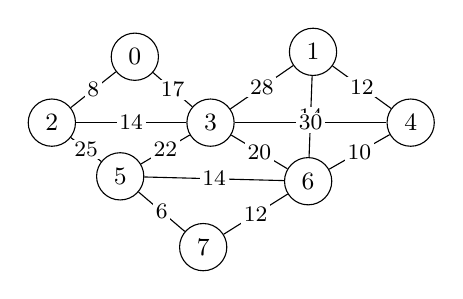
\begin{tikzpicture}[x=0.62cm, y=0.62cm,
    v/.style={circle, draw, minimum size=6mm, inner sep=0pt, font=\small},
    w/.style={fill=white, inner sep=1pt, font=\footnotesize}]
\node[v] (0) at (2.65,-0.9) {0};
\node[v] (1) at (6.3,-0.8) {1};
\node[v] (2) at (0.95,-2.25) {2};
\node[v] (3) at (4.2,-2.25) {3};
\node[v] (4) at (8.3,-2.25) {4};
\node[v] (5) at (2.35,-3.35) {5};
\node[v] (6) at (6.2,-3.45) {6};
\node[v] (7) at (4.05,-4.8) {7};
\draw (0) -- node[w] {8} (2);
\draw (0) -- node[w] {17} (3);
\draw (2) -- node[w] {14} (3);
\draw (1) -- node[w] {28} (3);
\draw (1) -- node[w] {12} (4);
\draw (1) -- node[w] {14} (6);
\draw (3) -- node[w] {30} (4);
\draw (2) -- node[w] {25} (5);
\draw (3) -- node[w] {22} (5);
\draw (3) -- node[w] {20} (6);
\draw (5) -- node[w] {14} (6);
\draw (6) -- node[w] {10} (4);
\draw (5) -- node[w] {6} (7);
\draw (7) -- node[w] {12} (6);
\end{tikzpicture}
\end{center}
\begin{enumerate}[leftmargin=2.2em]
\item[㈠] 分別使用相鄰矩陣（adjacency matrix）與相鄰串列（adjacency list）來儲存此圖時，何者所需之記憶
體空間較小？假設節點編號與邊值均不大於 255，且指標欄位需占用 4 個位元組（byte）。（5 分）
\item[㈡] 利用 Sollin 演算法（Sollin's Algorithm）找出此圖的最小成本生成樹（minimum cost spanning tree），
須按步驟寫出此樹的成長過程。（7 分）
\end{enumerate}
\end{pastexam}

\begin{pastsoln}
圖有 8 個頂點、14 條邊（無向）：(0,2) 8、(0,3) 17、(1,3) 28、(1,4) 12、(1,6) 14、(2,3) 14、(2,5) 25、
(3,4) 30、(3,5) 22、(3,6) 20、(4,6) 10、(5,6) 14、(5,7) 6、(6,7) 12。

\textbf{㈠ 相鄰矩陣比較省。} 編號和成本都不大於 255，各用 1 個位元組存（資結書第~21.2~節）。
\begin{itemize}
\item \textbf{相鄰矩陣}：$8 \times 8$ 個元素，每格存成本（0 表示沒有邊），每格 1 位元組，共
$64$ 位元組。
\item \textbf{相鄰串列}：8 個串列開頭指標，每個 4 位元組，共 32 位元組。 無向圖每條邊在兩端的串列
各出現一次，共 $2 \times 14 = 28$ 個節點；每個節點存鄰居編號（1 位元組）、成本（1 位元組）和
指向下一個節點的指標（4 位元組），共 6 位元組，$28 \times 6 = 168$ 位元組。 合計 $32 + 168 = 200$
位元組。
\end{itemize}
$64 < 200$，相鄰矩陣所需空間較小。 原因是指標占 4 位元組，比資料本身大得多，而這張圖邊不算少
（14 條，最多 28 條），串列省下的空格抵不過指標的成本。 （若矩陣只存上三角，只要 28 位元組，差距更大。）

\textbf{㈡ Sollin 演算法。} 每一回合，目前森林裡的每一棵樹（元件）各自挑「連到別的元件的最輕的邊」，
全部一起加入，元件兩兩合併；重複到只剩一個元件（資結書第~24.4~節）。 一開始每個頂點自己是一個元件。

\textbf{第 1 回合}：每個頂點挑最輕的邊。
\begin{center}
\begin{tabular}{cll}
\toprule
頂點 & 相連的邊 & 挑選 \\
\midrule
0 & (0,2) 8, (0,3) 17 & (0,2) 8 \\
1 & (1,3) 28, (1,4) 12, (1,6) 14 & (1,4) 12 \\
2 & (0,2) 8, (2,3) 14, (2,5) 25 & (0,2) 8 \\
3 & (0,3) 17, (1,3) 28, (2,3) 14, (3,4) 30, (3,5) 22, (3,6) 20 & (2,3) 14 \\
4 & (1,4) 12, (3,4) 30, (4,6) 10 & (4,6) 10 \\
5 & (2,5) 25, (3,5) 22, (5,6) 14, (5,7) 6 & (5,7) 6 \\
6 & (1,6) 14, (3,6) 20, (4,6) 10, (5,6) 14, (6,7) 12 & (4,6) 10 \\
7 & (5,7) 6, (6,7) 12 & (5,7) 6 \\
\bottomrule
\end{tabular}
\end{center}
不重複的邊有 (0,2) 8、(1,4) 12、(2,3) 14、(4,6) 10、(5,7) 6 五條，全部加入。 元件變成
$\{0, 2, 3\}$、$\{1, 4, 6\}$、$\{5, 7\}$。

\textbf{第 2 回合}：每個元件挑連到外面最輕的邊。
\begin{itemize}
\item $\{0, 2, 3\}$：往外的邊有 (1,3) 28、(3,4) 30、(2,5) 25、(3,5) 22、(3,6) 20，挑 (3,6) 20。
\item $\{1, 4, 6\}$：(1,3) 28、(3,4) 30、(3,6) 20、(5,6) 14、(6,7) 12，挑 (6,7) 12。
\item $\{5, 7\}$：(2,5) 25、(3,5) 22、(5,6) 14、(6,7) 12，挑 (6,7) 12。
\end{itemize}
不重複的邊 (3,6) 20、(6,7) 12，加入後三個元件合成一個，結束。

\textbf{成長過程}：
\begin{center}
\begin{tikzpicture}[x=0.5cm, y=0.5cm,
    v/.style={circle, draw, minimum size=5mm, inner sep=0pt, font=\scriptsize},
    w/.style={fill=white, inner sep=0.5pt, font=\scriptsize}]
\foreach \dx/\stage in {0/1, 11/2}{
\begin{scope}[xshift=\dx cm*0.5]
\node[v] (0) at (2.65,-0.9) {0};
\node[v] (1) at (6.3,-0.8) {1};
\node[v] (2) at (0.95,-2.25) {2};
\node[v] (3) at (4.2,-2.25) {3};
\node[v] (4) at (8.3,-2.25) {4};
\node[v] (5) at (2.35,-3.35) {5};
\node[v] (6) at (6.2,-3.45) {6};
\node[v] (7) at (4.05,-4.8) {7};
\draw[very thick] (0) -- node[w] {8} (2);
\draw[very thick] (2) -- node[w] {14} (3);
\draw[very thick] (1) -- node[w] {12} (4);
\draw[very thick] (6) -- node[w] {10} (4);
\draw[very thick] (5) -- node[w] {6} (7);
\ifnum\stage=2
\draw[very thick] (3) -- node[w] {20} (6);
\draw[very thick] (7) -- node[w] {12} (6);
\fi
\node[font=\small] at (4.6,-6) {第 \stage{} 回合後};
\end{scope}
}
\end{tikzpicture}
\end{center}
最小成本生成樹的邊：(0,2) 8、(2,3) 14、(1,4) 12、(4,6) 10、(5,7) 6、(3,6) 20、(6,7) 12，共
$n - 1 = 7$ 條，總成本 $8 + 14 + 12 + 10 + 6 + 20 + 12 = 82$。 用 Kruskal 檢查也得到 82。

本題第 1 回合每個頂點的最輕邊都沒有平手，第 2 回合 $\{1,4,6\}$ 和 $\{5,7\}$ 挑到同一條 (6,7)，
只加一次。 權重有平手時要固定一個比較規則（例如權重相同比編號），否則同時加入的邊可能成環
（資結書第~24.4~節）。
\end{pastsoln}
